
\section{Introdução}

\noindent \begin{minipage}[c]{0.6\textwidth}
  \vspace {1cm}
  \par A presente aula prática tem como fim a exploração do software Weka\ref{fig:logo_weka}, para a criação de uma rede neural Perceptron para interpretar corretamente os diferentes tipos de saídas do modelo.
  \par Para este fim é proposto o uso do software \href{https://www.cs.waikato.ac.nz/ml/index.html}{Weka}\ref{fig:logo_weka}, desenvolvido pela universidade do \href{https://www.waikato.ac.nz/}{Waikato} da Nova Zelândia, de acordo com \citeonline{Weka:2023}, o projeto possui quatro objetivos:
  \begin{asparaenum}
    \item tornar as técnicas de ML geralmente disponíveis;
    \item aplicá-los a problemas práticos importantes para a indústria da Nova Zelândia;
    \item desenvolver novos algoritmos de aprendizado de máquina e distribuí-los ao mundo;
    \item contribuir para um arcabouço teórico para a área.
  \end{asparaenum}

\end{minipage}
\begin{minipage}[c]{0.4\textwidth}

  
\includegraphics[width=\textwidth]{figure/weka-logo.jpg}
  	\label{fig:logo_weka}
    \captionof{figure}{Weka, \cite{Weka:2023}}
    %\captionof*{figure}{Fonte: \citeonline{linux:2023}}
\end{minipage}


\section{Métodos}
\par Os métodos aplicados nesta aula prática foi seguido o roteiro da \href{https://github.com/OgliariNatan/neuralPerceptron/blob/main/Aula%20pr%C3%A1tica.pdf}{aula prática}, no roteiro da presente aula, foi deixado em aberto os passos para a instalação do software Weka. Em consulta rápida na internet encontrei um documento publico denominado de \href{https://github.com/OgliariNatan/neuralPerceptron/blob/main/ML-09weka.pdf}{"Introdução ao Weka"}, da universidade federal do Paraná. do autor David Menotti. Segui as orientação e conclui a instalação do software como demonstra a figura \ref{fig:home_weka}.
\begin{figure}[h]
  \center
  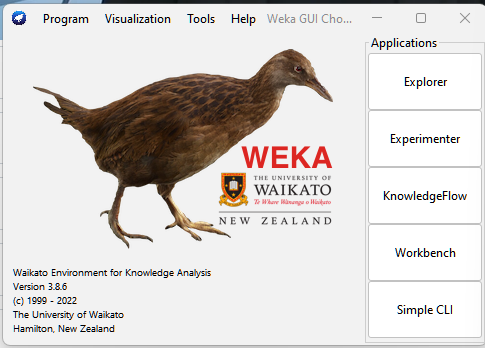
\includegraphics[scale=0.5]{figure/home_weka.png}
  \caption{Página inicial do Weka, O autor}\label{fig:home_weka}
\end{figure}
\par De acordo com o software, a versão instalada foi a \textbf{3.8.6}


%%%%%%%%%%%%%%%%%%%%%%%%%%%%%%%%%%%%%%%%%%%%%%%%%%%%%%%%%%

\section{Resultados}

\begin{figure}[H] %Figuras da aula pratica 1.1
  \center
  \subfigure[Perceptron.\label{fig:frist}]{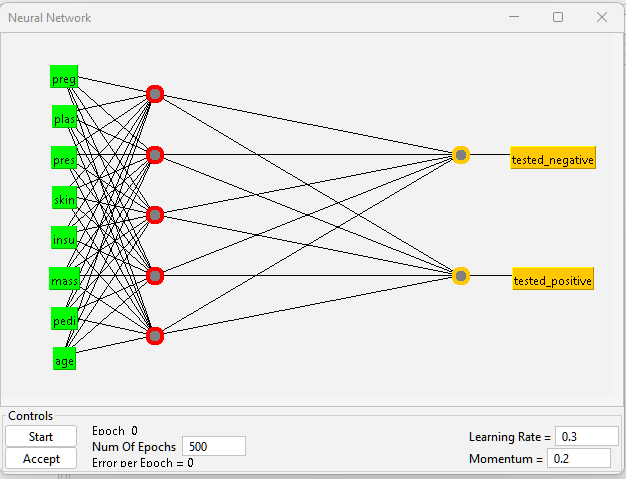
\includegraphics[scale=0.6]{figure/result.png}}

  \subfigure[Perceptron 75\%.\label{fig:75}]{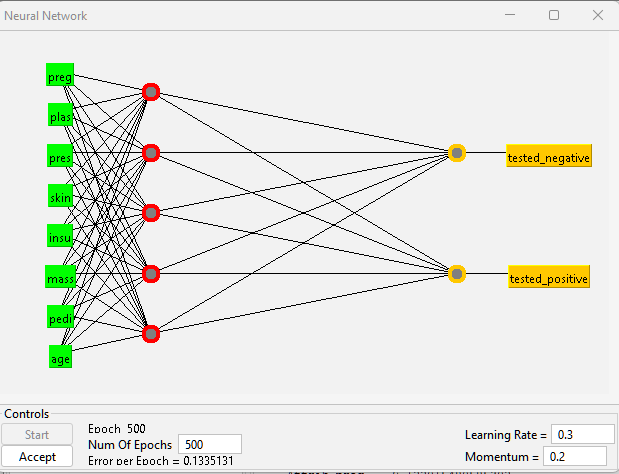
\includegraphics[scale=0.6]{figure/result_75p.png}}
  \caption{Rede neural Perceptron, O autor}\label{fig:redeNeural}
\end{figure}

%%%%%%%%%%%%%%%%%%%%%%%%%%%%%%%%%%%%%%%%%%%%%%%%%%%%%%%%%%%%%%%%%%%%%%%%%%%%%%%%%%%%%%%
\section{Conclusões}




  %$X \xLongleftarrow[\text{NATAN}]{\text{OGLIARI}} Y $ %COM TEXTO
	% $\uparrow$ %Seta para Cima
	%$\overleftarrow{NATAN}$
